\section{Introduction}
\label{sec:1}
An underlay cognitive radio system (\myUCRS{}) aims at finding spectrally efficient and low-latency ultra reliable transmission methods required to meet an increasing number of users and wireless technologies. In \myUCRS{}, an \mySU{} is allowed to transmit along with a \myPU{} subject to certain interference constraints. The spectral efficiency (\mySE{}) of the \mySU{} (for short the \mySE{} in the sequel) can be increased by using a cross-layer optimization (\myCLO{}) approach which optimizes the \mySU{} transmission parameters and employs an automatic repeat request (\myARQ{}) protocol subject to required quality-of-service (\myQoS{}) constraints of the \mySU{} and interference constraints of the \myPU{}. Here, on erroneous reception of transmission packets, the \mySU{} receiver (\myRX{}) can request the \mySU{} transmitter (\myTX{}) to retransmit the packet. A truncated hybrid \myARQ{} (\myTHARQ{}) type \myII{}, where chase combining (\myCC{}) is used to combine identical copies of erroneous packets for a predetermined maximum number of retransmissions, is a modification to a \myTHARQ{} type \myI{} where the latter discards previously detected packets.

The authors in~\cite{Park2016_alt} and~\cite{Wu2016_alt} discuss different implementations of \myARQ{} with \myCC{}. While~\cite{Wu2016_alt} analyses how an \myARQ{} can improve the reliability of transmission,~\cite{Park2016_alt} shows that symbol-level combining outperforms bit-level combining. \myCC{} provides a power gain for low-density parity check (\myLDPC{}) transmissions~\cite{Hoefel2021_alt}. A constrained Markov decision process for cross-layer packet scheduling using \myARQ{} is proposed in~\cite{Muttath2022_alt}. In~\cite{Shafique2016_alt}, a \myCLO{} is proposed for \myCC{} with orthogonal frequency-division multiplexing using selective retransmissions to improve the spectral efficiency (\mySE{}) without transmitting entire erroneous packets again. While the authors in \cite{Ramis2010_alt} and \cite{Ge2015_alt} propose \myCC{}-\myCLO{} schemes which strive to enhance the \mySE{} by optimizing the packet-error rate and payload length, respectively, the authors in \cite{Taricco2023_alt} and \cite{Fernando2023_alt} employ a similar architecture to optimize the power allocation of the \mySU{} transmission in 5G networks.
\begin{figure*}[!t] 
  \centering
  \begin{psfrags}
    \psfrag{err}[c][c]{\figtext{\myCRCcheck}}
    \psfrag{pa}[c][c]{\rotatebox{90}{\tiny \myFail}}
    \psfrag{fa}[l][l]{\hspace{-0.1cm}{\figtext{\myPass}}}
    \psfrag{at}[c][c]{\figtext{$\myBhatkhat$}}
    \psfrag{srx}[r][r]{\raisebox{0.5ex}{\figtext{\mySU{} \myRX{}}}}
    \psfrag{buffer}[c][c]{\rotatebox{90}{\figtext{buffer}}}
    \psfrag{ton}[c][c]{\raisebox{-0.2ex}{\scalebox{0.60}{\figtext{$1$}}}}
    \psfrag{two}[c][c]{\raisebox{-0.15ex}{\scalebox{0.70}{\figtext{$2$}}}}
    \psfrag{tj}[c][c]{\scalebox{0.80}{\figtext{$j$}}}
    \psfrag{dd}[c][c]{\raisebox{1.5ex}{\scalebox{0.50}{\rotatebox{150}{\myJDots}}}}
    \psfrag{pho}[c][c]{\figtext{\myCLO{}: \myPHY{} parameters}}
    \psfrag{feedpy}[c][c]{\raisebox{-0.2ex}{\figtext{feedback channel \myPHY{}}}}
    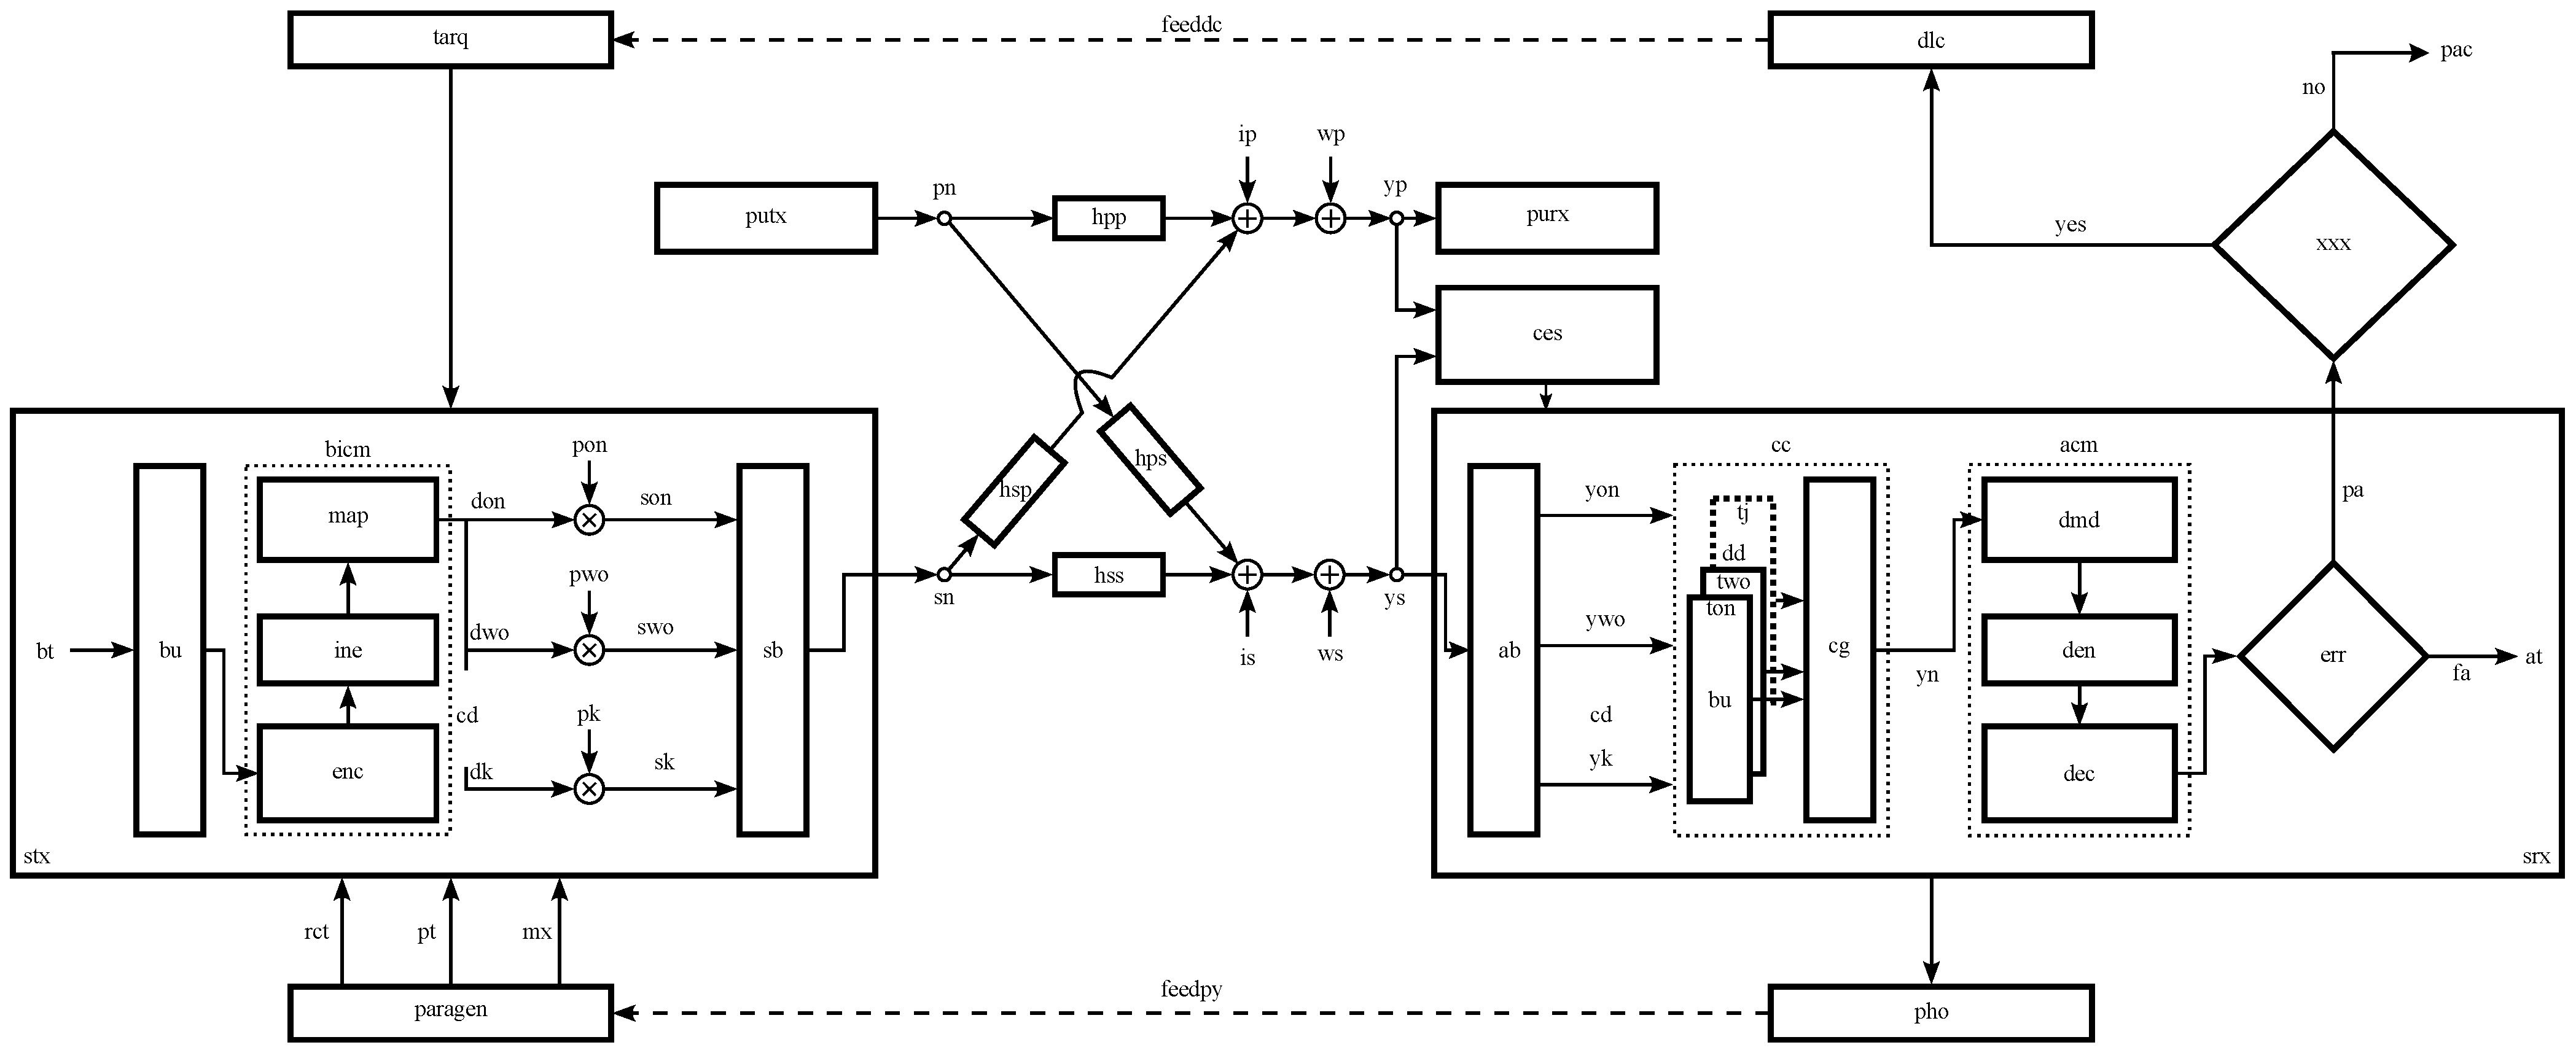
\includegraphics[width=\textwidth]{Figures/findraw_240101.eps}
  \end{psfrags}
  \caption{{\normalsize Underlay CR system model with cross-layer optimization and chase combining.}}
  \label{fig:1}
\end{figure*}

All these methods, however, do not consider any collective adaptation of coding and modulation schemes along with a \myCC{} implementation. The authors in \cite{Mansour2022_alt} propose a \myCLO{} of \myUCRS{} with a discrete Fourier transform modulated filter bank (\myDFTFB{}) using joint bit loading (\myBL{}) and power loading (\myPL)~(\myJBPL) coupled with coding adaptation (\myCA) and \myTHARQ{}. They employ bit-interleaving in combination with minimization of the uncoded bit-error-rate, which allows using different channel coding schemes to minimize coded bit-error-rate. A stochastic chance-constrained programming (\mySCP{}) \cite{Ding2012_alt} is applied to satisfy an interference constraint at the \myPU{} \myRX{} with a given confidence level.

In this paper, the work in~\cite{Mansour2022_alt} is extended as follows:
\vspace{0.5em}
\begin{itemize}[leftmargin=0.9em]
    \renewcommand\labelitemi{$\scriptstyle\bullet$}
    \item In \cite{Mansour2022_alt}, a \myTHARQ{} type \myI{} is considered where erroneous packets are discarded and no diversity or combination gains can be achieved, degrading the achievable \mySE{}. In this paper, a \myTHARQ{} type \myII{} operation with \myCC{} is considered to exploit diversity and combination gains to maximize the achievable \mySE{}.
    \item In~\cite{Mansour2022_alt}, convolutional coding is used in combination with puncturing, while in this paper an \myLDPC{} coding transmission is considered in combination with rate matching, providing better error-correction performance and lower error floors.
    \item The closed form of the lower bound on the \mySE{} in \cite{Mansour2022_alt} is extended and maximized considering \myLDPC{} coding and \myCC{} protocols subject to specific \myQoS{} and interference constraints, validated numerically.
\end{itemize}
\vspace{0.5em}

This paper is organized as follows. Sect.~\ref{sec:2} describes the \myUCRS{} with the \myDFTFB{}s using \myCLO{} and \myTHARQ{} under the influence of third-party interference (\myTPI{}) in addition to the \myPU{} signal. In Sect.~\ref{sec:3}, the \myCLO{} for coded \mySU{} transmission is presented with physical layer (\myPHY{}) and data link control layer (\myDLC{}) parameters. The \myCLO{} system performance is evaluated in Sect.~\ref{sec:4}. Conclusions are drawn in Sect.~\ref{sec:5}.

In this paper, vectors are represented by boldfaced characters and random variables (\myRV s) by capital letters. Furthermore, $\myE{\cdot}$, $\EX{X}{\cdot}$, $\inner{\cdot}{\cdot}$, and $\cond{X}{Y}{y}$ denote expectation, expectation with respect to the \myRV{} $\myX$, inner product, and an \myRV{} $\myX$ conditioned on the \myRV{} $\myY$ taking a value $\myY = \myy$, respectively. Parameters indexed by roman characters $\myPrm{}$, $\mySrm$, (\myun{}) and (\myco{}) are associated with the (\myPU{}), (\mySU{}), uncoded and coded transmissions, respectively. Finally, we define an index set $\Omegaset{a}{b}$ for $\mya \in \myZbb{}$ and $\myb \in \myNbb{}$.
